%\setlength{\headsep}{1.5cm} % Distância entre a margem superior do quadro do texto e o cabeçalho.
\chapter{RESULTS AND DISCUSSION }
\label{chapter:servidores_linux}
\vspace{-2cm}


Brazil is a country of continental dimensions with contrasting climates, which were represented by the chosen locations. The World Meteorological Organisation(WMO) establishes the general procedures to calculate the monthly 30 year standard normals and averages \cite{wmo1989calculation}, which are important climatological variables that describes the climatic conditions of a given location. This index were used to contradistinguish the high variability of climate conditions that the ANN structures had to handle. The two opposite climate conditions were Campo Mourão and Jaguaruana, the normals of both locations are represented by Fig. \ref{img:figure4}.


\begin{figure}[htbp]
\subfloat[Campo Mourão]{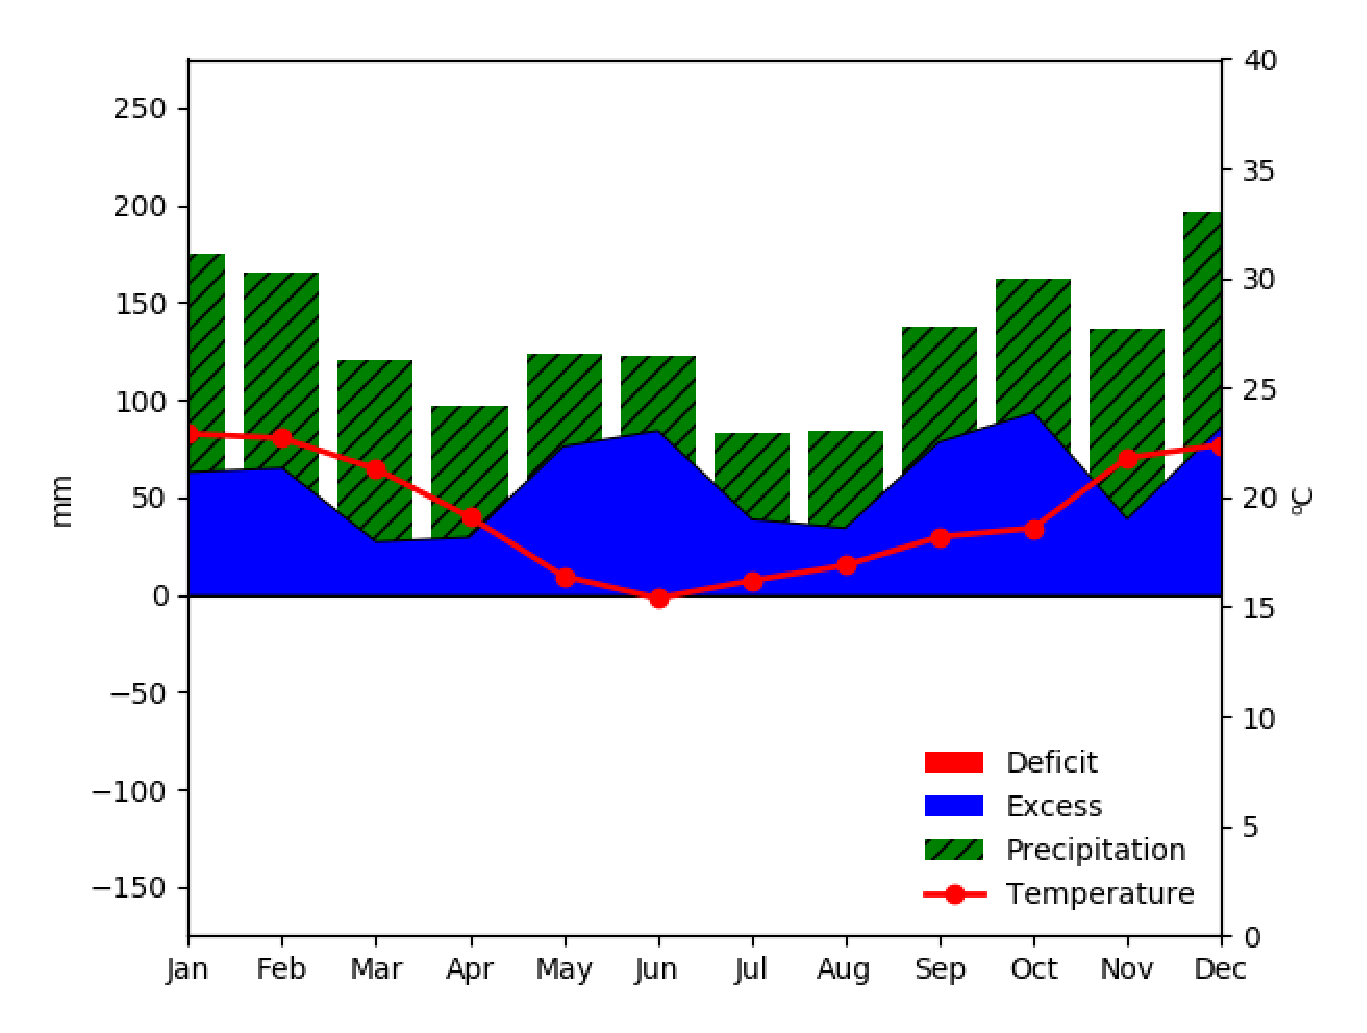
\includegraphics[scale=0.36]{capitulo_3/campo_moral_normal}}
\subfloat[Jaguaruana]{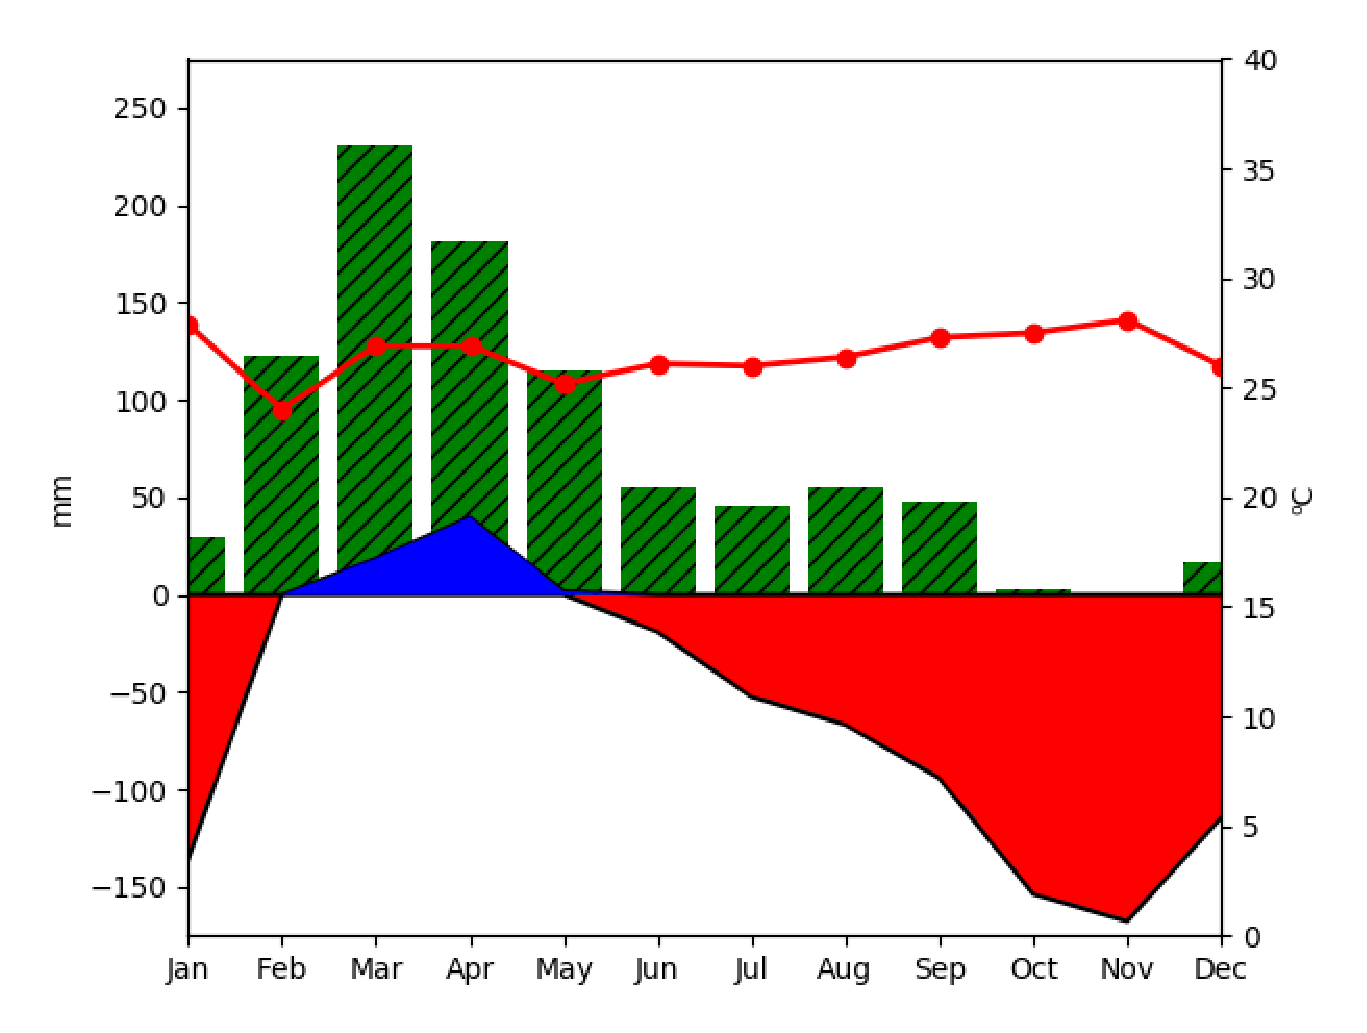
\includegraphics[scale=0.36]{capitulo_3/jaguaruana_normal}}
\caption{Thornthwaite Water Balance and Normal Temperature}
\label{img:figure4}
\end{figure}


Campo Mourão have an subtropical humid mesothermal weather with hot summers and not frequent frosts, the precipitation is well distributed with an accumulated volume of 1603 \textit{mm} there is allegedly no water deficit throughout the year, in contrast Jaguaruana have an tropical savanna climate with water deficit across the year with exception of the months from February to May with an accumulated precipitation of 906 \textit{mm}, the location is an  good representation of the Brazilian semi-arid region. Between these two contrasting climates there are the climes of all the other locations used in this paper, the climate of each location lays among the Jaguaruana tropical savanna and the Campo Mourão humid mesothermal weather. Given the conditions if it were used only one ANN structure for all locations and seasons the noise would be high, and both the accuracy and precision would decay. 

To summarise all the the ANNs assertiveness or the capacity to retrieve information in an general perspective, it was computed the mean accuracy percentage average for all locations for each time range($[3,...,7]$\textit{days}) and season. In the Fig. \ref{img:figure5} it is shown the summarisation both for the \textit{autoassociative} (a) and \textit{heteroassociative}(b) capabilities of the ANNs structures, the auto-association is the phenomenon of associating the input vector with itself as the output as called by estimation capacity, and the hetero-association is that of recalling a related vector given an input vector or the forecasting capacity \cite{rao1995c++}. 


\begin{figure}[htb!]
 \centering
 \subfloat[autoassociative]{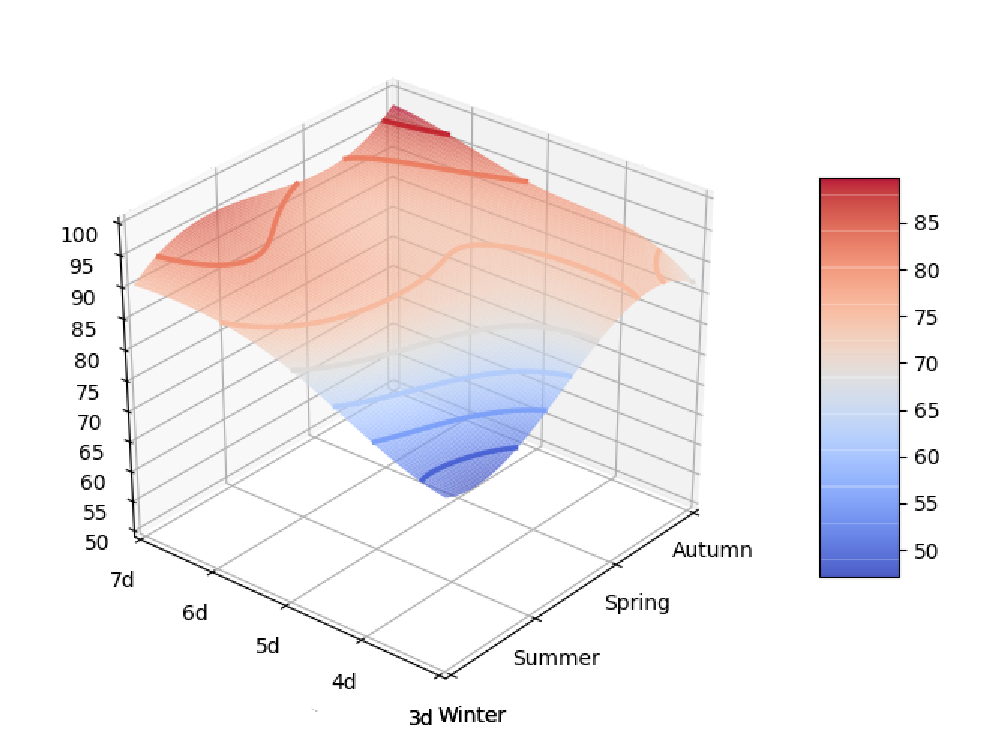
\includegraphics[scale=0.37]{capitulo_3/estimate_accuracy_2}}
 \subfloat[heteroassociative]{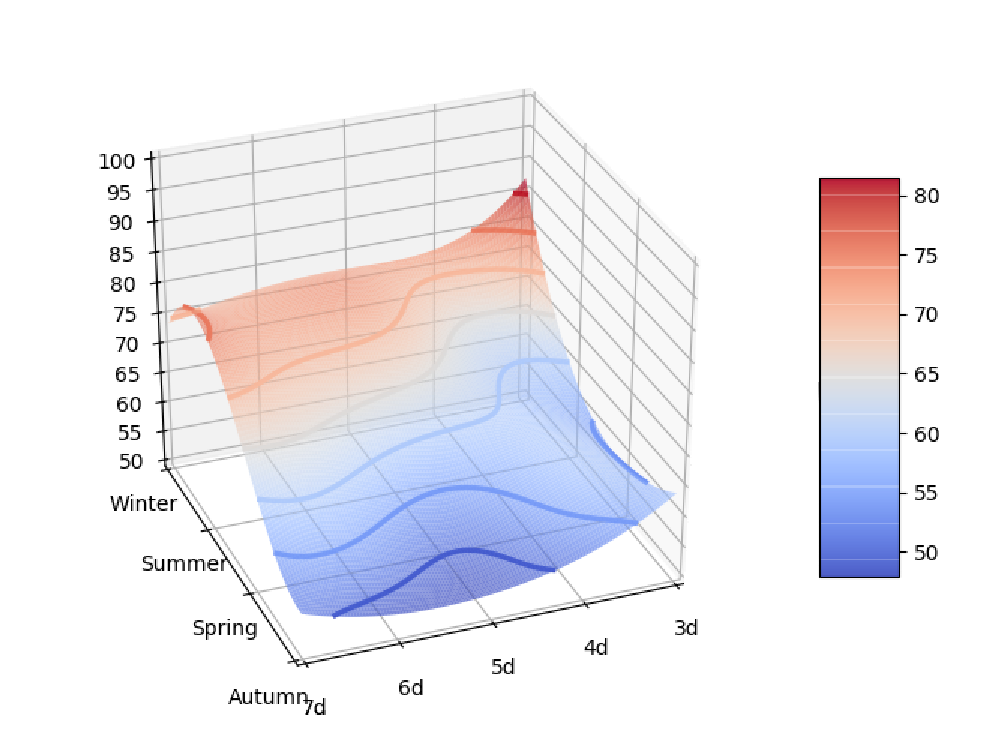
\includegraphics[scale=0.37]{capitulo_3/forecasting_accuracy2}}
 \caption{Summary of ANNs autoassociative (a) and heteroassociative(b) performance}
  \label{img:figure5}
\end{figure}


When trying to self associate, the less accurate ANN was the one trained with winter data for a cumulative period of three days and had an accuracy of 77.15\% for all regions, 
The most accurate were trained with autumn data and an period of seven days achieving a accuracy of 97.61\% , between all ANNs and cumulative periods the estimation performance average was of 89.18\% indicating that the ANN was able to recall the input variables and associate it with the desired output, which is an quality indicative of the chosen inputs variables.

Different from estimation, the forecasting performance had an increased performance variance, in its least accurate point which were in autumn with an accumulated period of 6 days, the ANN structure had an accuracy of 53.14\%, when most accurate it had an forecasting success of 87.14\% and were in winter with an 3 accumulated days. The Artificial Neural Networks that had the best performance were the ones that had their weights adjusted with data from winter and summer.  Relatively to other studies the performance was acceptable, Valipour et. al.\cite{valipour2016optimization} while detecting drought and wet years obtained an average correlation of 0.90, in the prediction stage the model was mostly accurate and dependant on the levels of deforestation. Rivero et. al. \cite{rivero2015short} developed a methodology based on ANNs to forecast rainfall on a monthly period with incomplete datasets, the author utilised the symmetric mean absolute percentage error(SMAPE) as a performance metric, the best performing model had an score of 0.51 which the author classifies as almost acceptable.

In Brazil on latitudes near the equator line like the city of Jaguaruana, winter is the time of year that the rainfall index is usually higher. In summer this index tend to fall, however at lower latitudes this indices reverse and winter happens to be the dry season of the year, in both situations the climate is well defined making it easier for the neural network to generalize its knowledge and accurately forecast the rainfall occurrence, winter in all the accumulated periods was the most predictable season.
  
Autumn and spring are transitional epochs and there is a mix of climate characteristics both from winter to summer, as from summer to winter. In these seasons the artificial neural networks notably had greater difficulty in forecasting clearly whether or not there would be rainfall, autumn was the least predictable season. 
Despite the forecast accuracy being smaller in both seasons this is an important result, it indicates that it was wise to create an model for each climate season, if this were not done and the general model have been divided into only 2 times of the year, this effect would have been diluted in the results vector, so that the shape of the forecast chart in Fig \ref{img:figure5} would become flattened. 

In the first half of the year of southern hemisphere are contained the summer and fall, the inability of the network to generalise its knowledge of autumn would have negatively impacted the summer forecast capacity, in the second half of the year the effect would have been the same with the difference that the forecasting ability of winter would be impacted by the spring. In the Fig. \ref{img:figure6} is shown the detailed performance of each ANN with an colour scale that visually represents the relative accuracy of the model, by this figure is clear the predominance of the ANNs models being more accurate both on summer and winter, the combination of location and season with the most notable performance was maceio on winter and the worst was Campo Mourão on autumn.  

\begin{figure}[htb!]
 \centering
  \caption{ANNs accuracy percentage performance}
 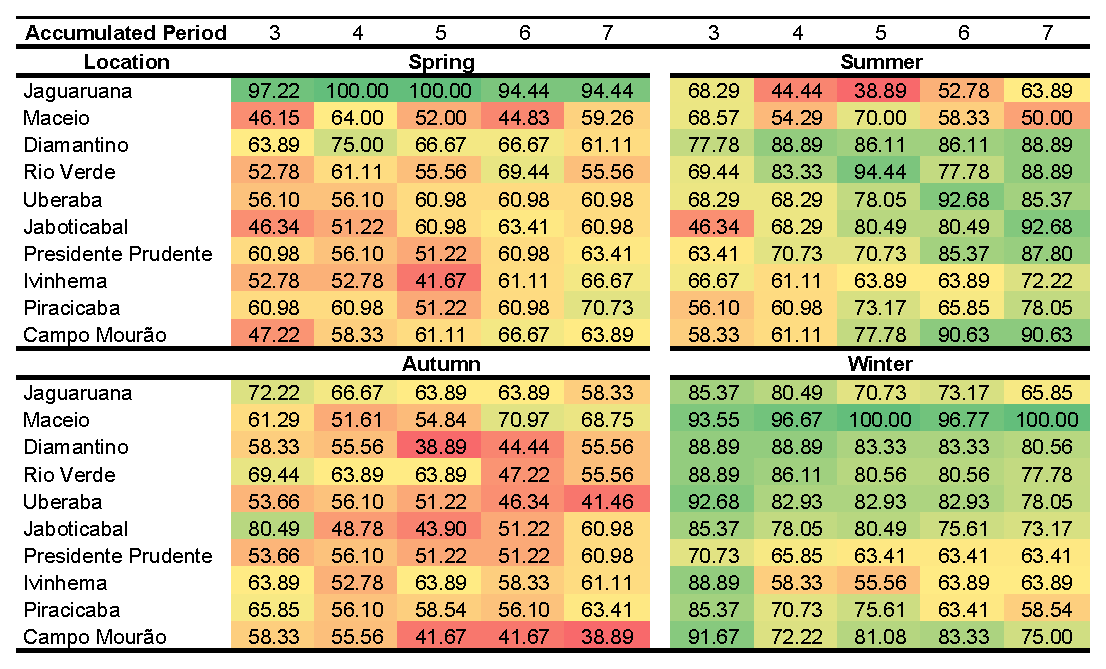
\includegraphics[scale=0.60]{capitulo_3/general_table}
 \label{img:figure6}
\end{figure}

When oceanic air masses moves to continent inland they loose water through precipitation and the remaining of this masses become progressively depleted in water vapour, this phenomena can be called continentality effect. By reaching orographic obstacles, the condensation and rainfall associated with the adiabatic cooling of these raising air masses and further deplete the vapor of it, which is called altitude effect \cite{vuille2003modeling}. The continentality and altitude effect therefore can be important as sources of rainfall variability over the years and as shown by Fig.\ref{img:figure7} and Fig. \ref{img:figure8} impact on the ANNs prediction performance. 


\begin{figure}[htb!]
 \centering
  \caption{The effect of continentality on the ANNs accuracy at all seasons.}
 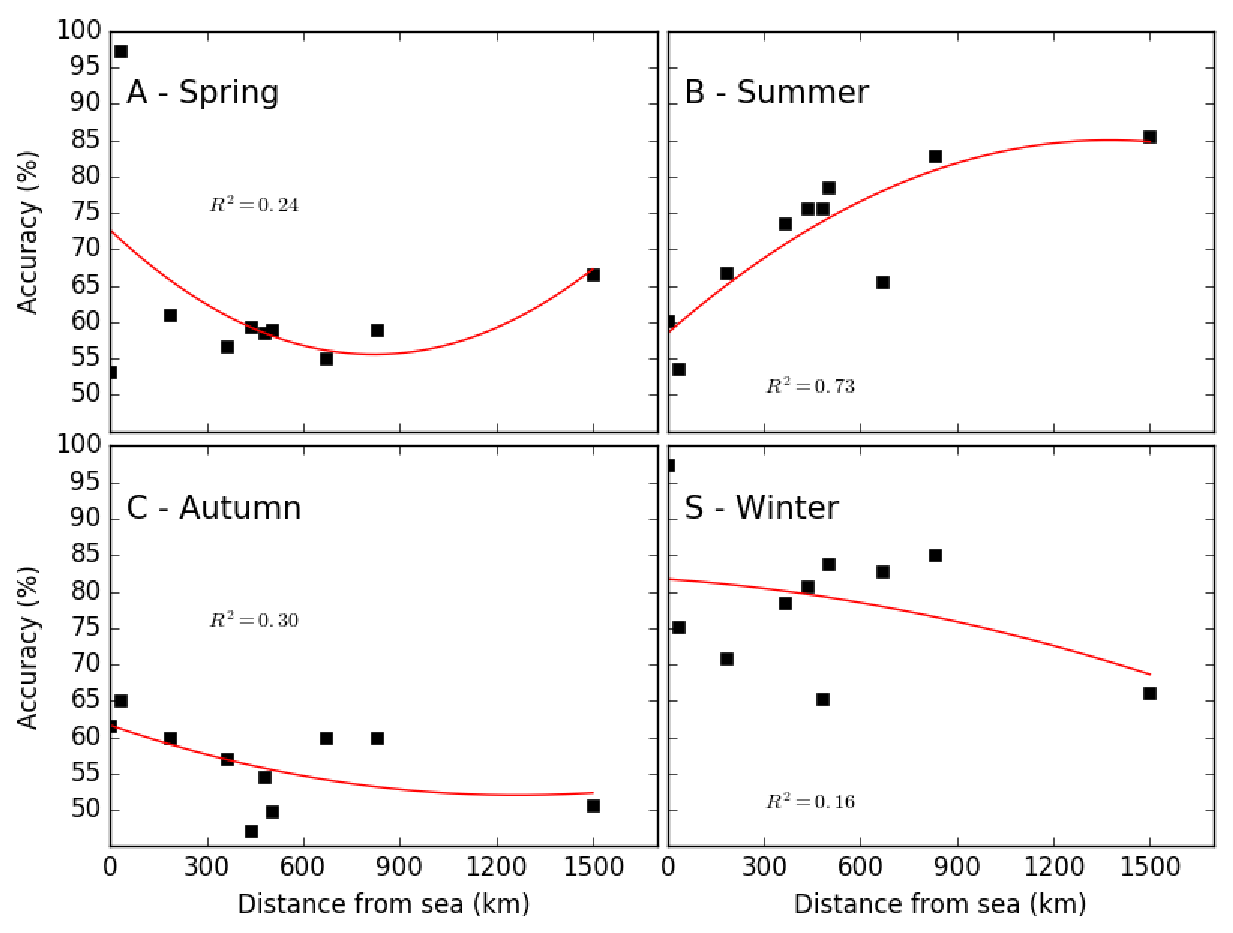
\includegraphics[scale=0.56]{capitulo_3/continentality_effect}
 \label{img:figure7}
\end{figure}
\begin{figure}[htb!]
 \centering
  \caption{The effect of altitude on the ANNs accuracy at all seasons.}
 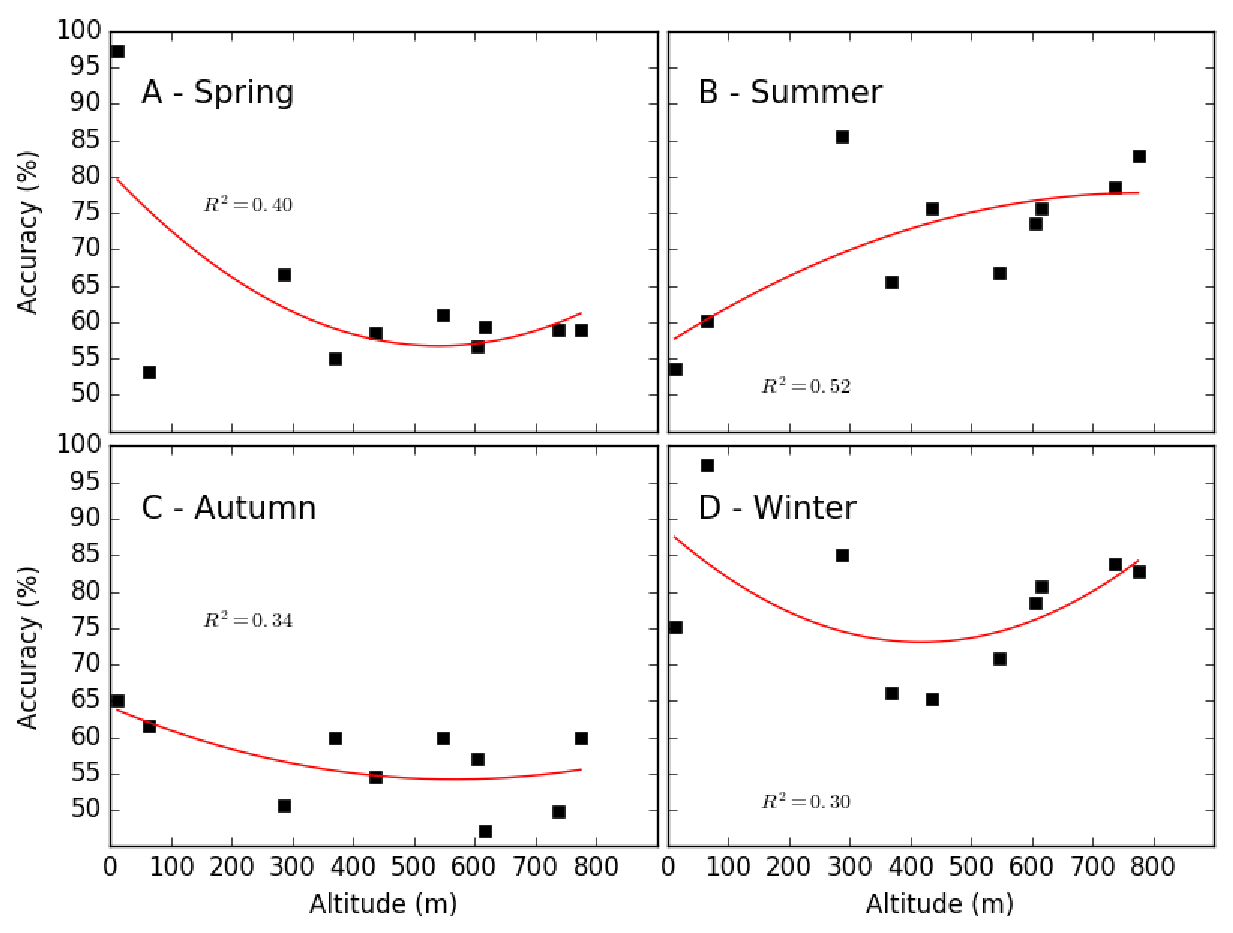
\includegraphics[scale=0.56]{capitulo_3/topographic_effect}
 \label{img:figure8}
\end{figure}

\newpage
The Continentality effect was a more prominent source of noise to the ANNs at summer, the closer to the sea the bigger it was the impact on the ANNs accuracy which is actually coherent. Summer is the season that the amount of solar radiation and energy in the atmosphere are higher and consequently the amount of oceanic air masses coming inward are greater. These air masses are highly unstable closer to the sea and tend to loose its strength and stabilise as they move into the continent, the impact of this phenomena on the ANNs forecasting accuracy is represented in the Fig. \ref{img:figure7} graph B.

On winter the effect of continentality on the ANNs is quite the opposite of what happens on summer, mainly because the amount of maritime air masses is lower than summer which reduces the climatic variability and reverses accuracy tendency of the ANNs as shown in the graph D of Fig. \ref{img:figure7}. As spring and autumn are transitional seasons the effect of continentality is not quite well defined, on the first half of spring the oceanic air masses behaves more like the ones of winter and on the second half it starts to behaves as the masses of summer, inverting this behaviour on autumn, the effect of continentality on this seasons are shown on graphs A and C of Fig. \ref{img:figure7}. Alvares et al. \cite{alvares2013modeling} described an strong correlation of temperature and the effect of continentality during summer and the opposite on winter which corroborate with the result obtained. 

The Altitude effect on summer behaves closely as the effect of continentality, there is a large amount of steam loaded air masses coming from sea and an increased amount of orographic rainfalls \cite{salati1979recycling} which is apparently a type of precipitation that the ANNs were able of correctly predict as shown by graph B of Fig \ref{img:figure8}. The altitude effect is not as prominent on the accuracy of the ANNs on winter (Fig.\ref{img:figure9} graph D) of which the amount of orographic rainfalls is quite reduced in comparison of summer, and both on spring and autumn it behaves as the continentality effect and by the same reasons. Other studies \cite{gonfiantini2001altitude} on tropical rains described an seasonal variation on rainfall volumes duo to altitude effect being more positive on summer with respects to winter. This seasoned influence is explained duo to the lowering of temperatures and consequent increase of the condensation rate of atmospheric vapour and a greater availability of air moisture on summer when compared to winter .

\begin{figure}[htb!]
 \centering
  \caption{The effect of precipitation volumes on ANN models}
 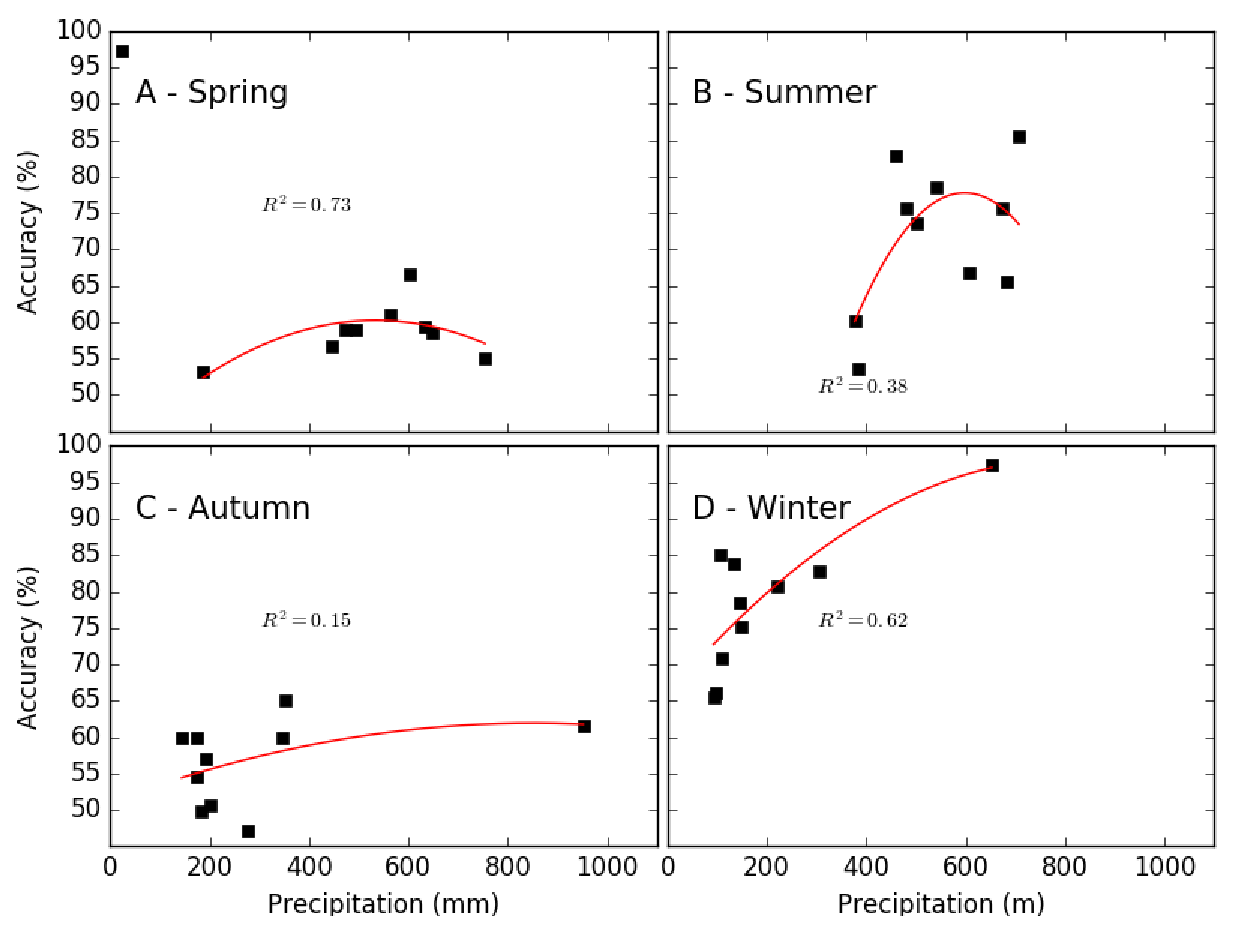
\includegraphics[scale=0.60]{capitulo_3/precipitation_accuracy}
 \label{img:figure9}
\end{figure}

One factor that can affect directly the ANNs accuracy is the rainfall frequency and volume by itself of which lack of exposure to a significant number of rainfall events can make the ANN underforecast and miss its occurrence \cite{kuligowski1998experiments}. As show by Fig. \ref{img:figure9} graphs B and D, on winter and summer the ANNs forecasting accuracy is correlated with the amount of rainfall in the period of which the accuracy of the model increases with the precipitation amount. In spring and autumn the precipitation volume do not affect the accuracy of the model. 

Comparing the results of this paper with previous studies \cite{kumarasiri2006rainfall, kuligowski1998experiments, nasseri2008optimized, hall1999precipitation, ramirez2006linear, rajurkar2002artificial} was difficult firstly because of the disparity of ranges of these studies, some have used short forecasting periods on the scale of hours and others used a monthly scale, secondly these studies were focused on predicting not only the rainfall event but also the precipitation volume, which wasn't the goal of this research. 
















